\section{Background}
Here we review some of the necessary mathematics behind the problem.  The
definitions found in this chapter are those found in 
\cite{kleinberg2006algorithm,demaine2008geometric,stephenson2005introduction,frederickson1997dissections}.
%\subsubsection{SAT to 3-SAT Gadget}
\subsection{SAT Problems}

\begin{prob}[Satisfiability Problem]\label{prob:ncpi-6}%Problem/Question
Let $\left\lbrace x_i \right\rbrace_{i=1}^{n} $ be boolean variables, and $t_i \in \left\lbrace x_i\right\rbrace_{i=1}^{n}  \cup \left\lbrace \bar{x}_i\right\rbrace_{i=1}^{n}   $.  A \textit{clause} is is said to be a disjuction of distinct terms:
$$
t_1 \vee \cdots \vee t_{j_k} = C_k
$$
Then the \textit{satisfiability problem} is the decidability of a conjuction of a set of clauses, i.e.:
$$ \wedge_{i=1}^m C_i$$
\end{prob} \cite{skiena2009algorithm}
\subsubsection{3-SAT Problems}
A 3-SAT problem is a SAT problem with all clauses having only three boolean variables. 
% \paragraph{Converting SAT to 3-SAT}
% \begin{itemize}
% \item[\rn{1}] Given a clause, $t_1 \vee t_2 \vee t_3 \vee \cdots \vee t_n$.
% \item[\rn{2}] Transform the clause given in (\rn{1}) to a conjuction of clauses as the following:
% $$\left( t_1 \vee t_2 \vee x_2 \right)\wedge\left( \bar{x}_2 \vee t_3 \vee x_3 \right)\wedge\left( \bar{x}_3 \vee t_4 \vee x_4 \right)\wedge \cdots \wedge \left( \bar{x}_{n-2} \vee t_{n-1} \vee t_n \right)$$
% \item[\rn{3}] Clauses with less than three boolean variables and be rewritten as $$\left( t_1 \vee x \vee \bar{x} \right) $$ or $$\left( t_1 \vee t_2 \vee x \right)\wedge \left( \bar{x}  \vee y \vee \bar{y} \right)$$
% \end{itemize}  
\subsection{Linkages}
\begin{definition}[Linkage]\label{def:linkages-1}
A collection of fixed-length 1D segments joined at their endpoints to form a graph.
\end{definition} 
\begin{definition}[Graph]\label{def:linkages-2}
An ordered pair $G = (V, E)$ comprising a set $V$ of vertices or nodes together with a set $E$ of edges or lines
\end{definition} 
\begin{definition}[Cycle]\label{def:linkages-3}
 A closed walk with no repetitions of vertices or edges allowed, other than the repetition of the starting and ending vertex
\end{definition} 
\begin{definition}[Configuration]\label{def:linkages-6}
A specification of the location of all the link endpoints, link orientations and
joint angles.\cite{demaine2008geometric}
\end{definition} 
\subsection{Dissections}
\begin{prob}[Polygonal Dissection]\label{def:dissection}
Given two polygons of equal area, $P_1$ and $P_2$, partition $P_1$ into smaller
pieces,$\left\lbrace P_{1,i}\right\rbrace_{i=1}^n $, rearrange the pieces to
form $P_2$. /cite{frederickson1997dissections}
\end{prob}
\begin{figure}[h]
\begin{center}
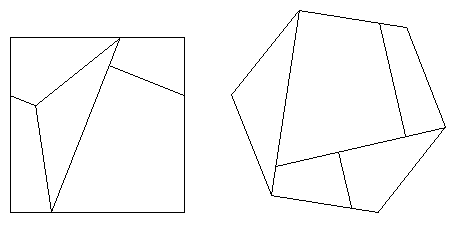
\includegraphics[scale=1]{graphics/polygonaldissection.png}
\caption{An axample of two polygons of equal area that can be rearranged into
the other by the given partition.\cite{davidEppstienJunkyard}}
\label{fig:polygonaldissection}
\end{center}
\end{figure}
\subsection{Circle Packing}
\begin{definition}[Circle Packing]\label{def:circlePacking}
$P$ of a planar graph $G$ is a set of of circles with disjoint
interiors $\left\lbrace C_v \right\rbrace_{v \in G} $ such that two
circles are tangent if and only if the corresponding vertices form an edge.
\cite{arXiv13113363v1}
\end{definition} 


\begin{thm}[Circle Packing Theorem]\label{thm2-1}
For every connected simple planar graph $G$ there is a circle packing in the
plane whose intersection graph is (isomorphic to) $G$.
\cite{stephenson2005introduction}
\end{thm}
\subsubsection{Circle Packings and Polygonal Linkages}
Given a circle of radius $r$, we establish the isomorphism to a hexagon by
circumscribing the vertices of the regular hexagon.
\begin{figure}[h]
\begin{center}
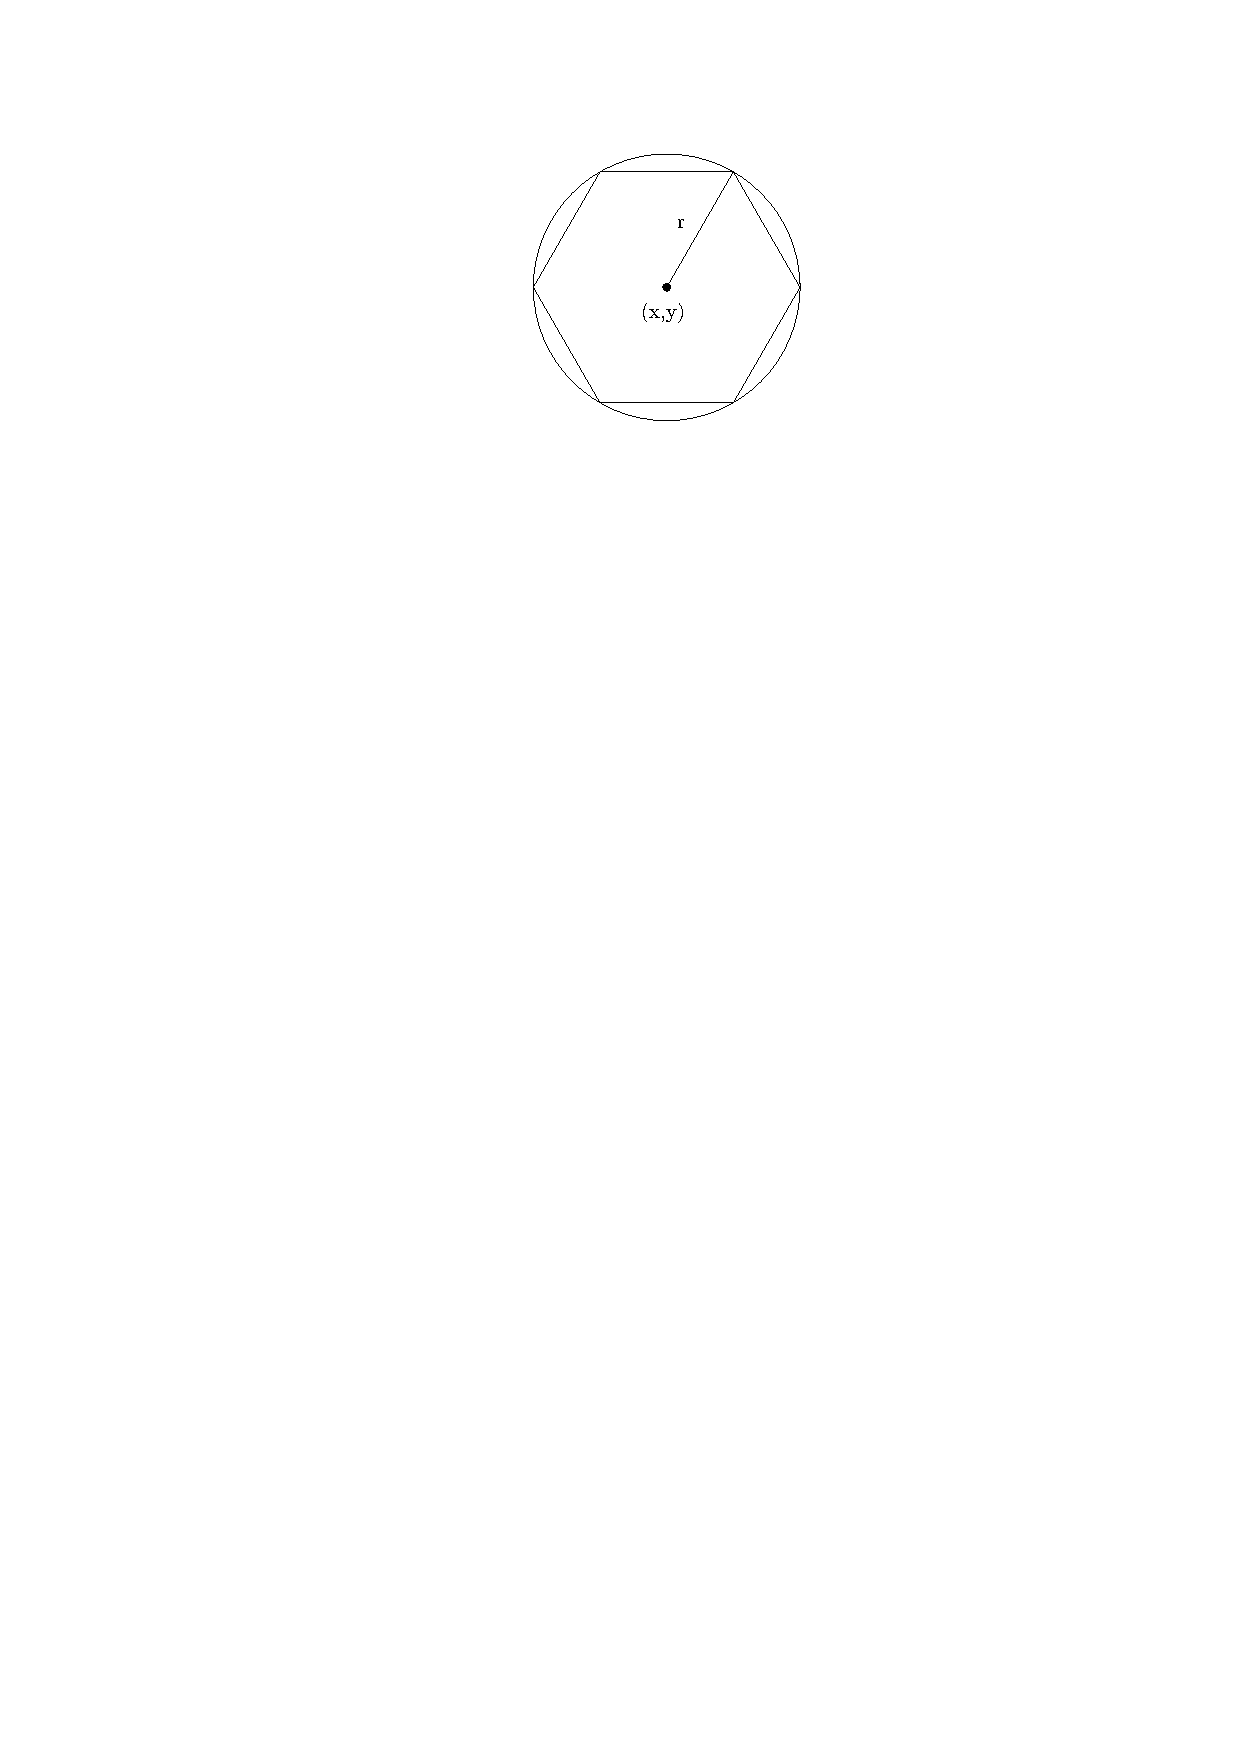
\includegraphics{graphics/circumscribedHexagon.pdf}
\caption{A circumbscribed hexagon}
\end{center}
\end{figure}
\subsubsection{Hinged Polygons}
\begin{definition}[Polygonal Chain]\label{def}
A polygonal chain $P = \left( v_0, v_1, \dots, v_{n-1}\right) $ is a sequence of
consecutively joined segments (or edges) $e_i = v_i v_{i+1}$ of fixed lengths
$l_i = \left\vert e_i\right\vert $, in a plane. \cite{Biedl99lockedand}
\end{definition}
A chain is said to be closed if $v_{n-1} = v_1$, otherwise it is said to be
open. Hinged polygons have been researched for decades and related to linkage problems
\cite{Biedl99lockedand,canny1988complexity}.

 Consider the locked configuration of figure \ref{figure:7hexLocked}.  We can
 configure the hexagons to be locked by placing hing points as follows:
\begin{figure}[h]
\begin{center}
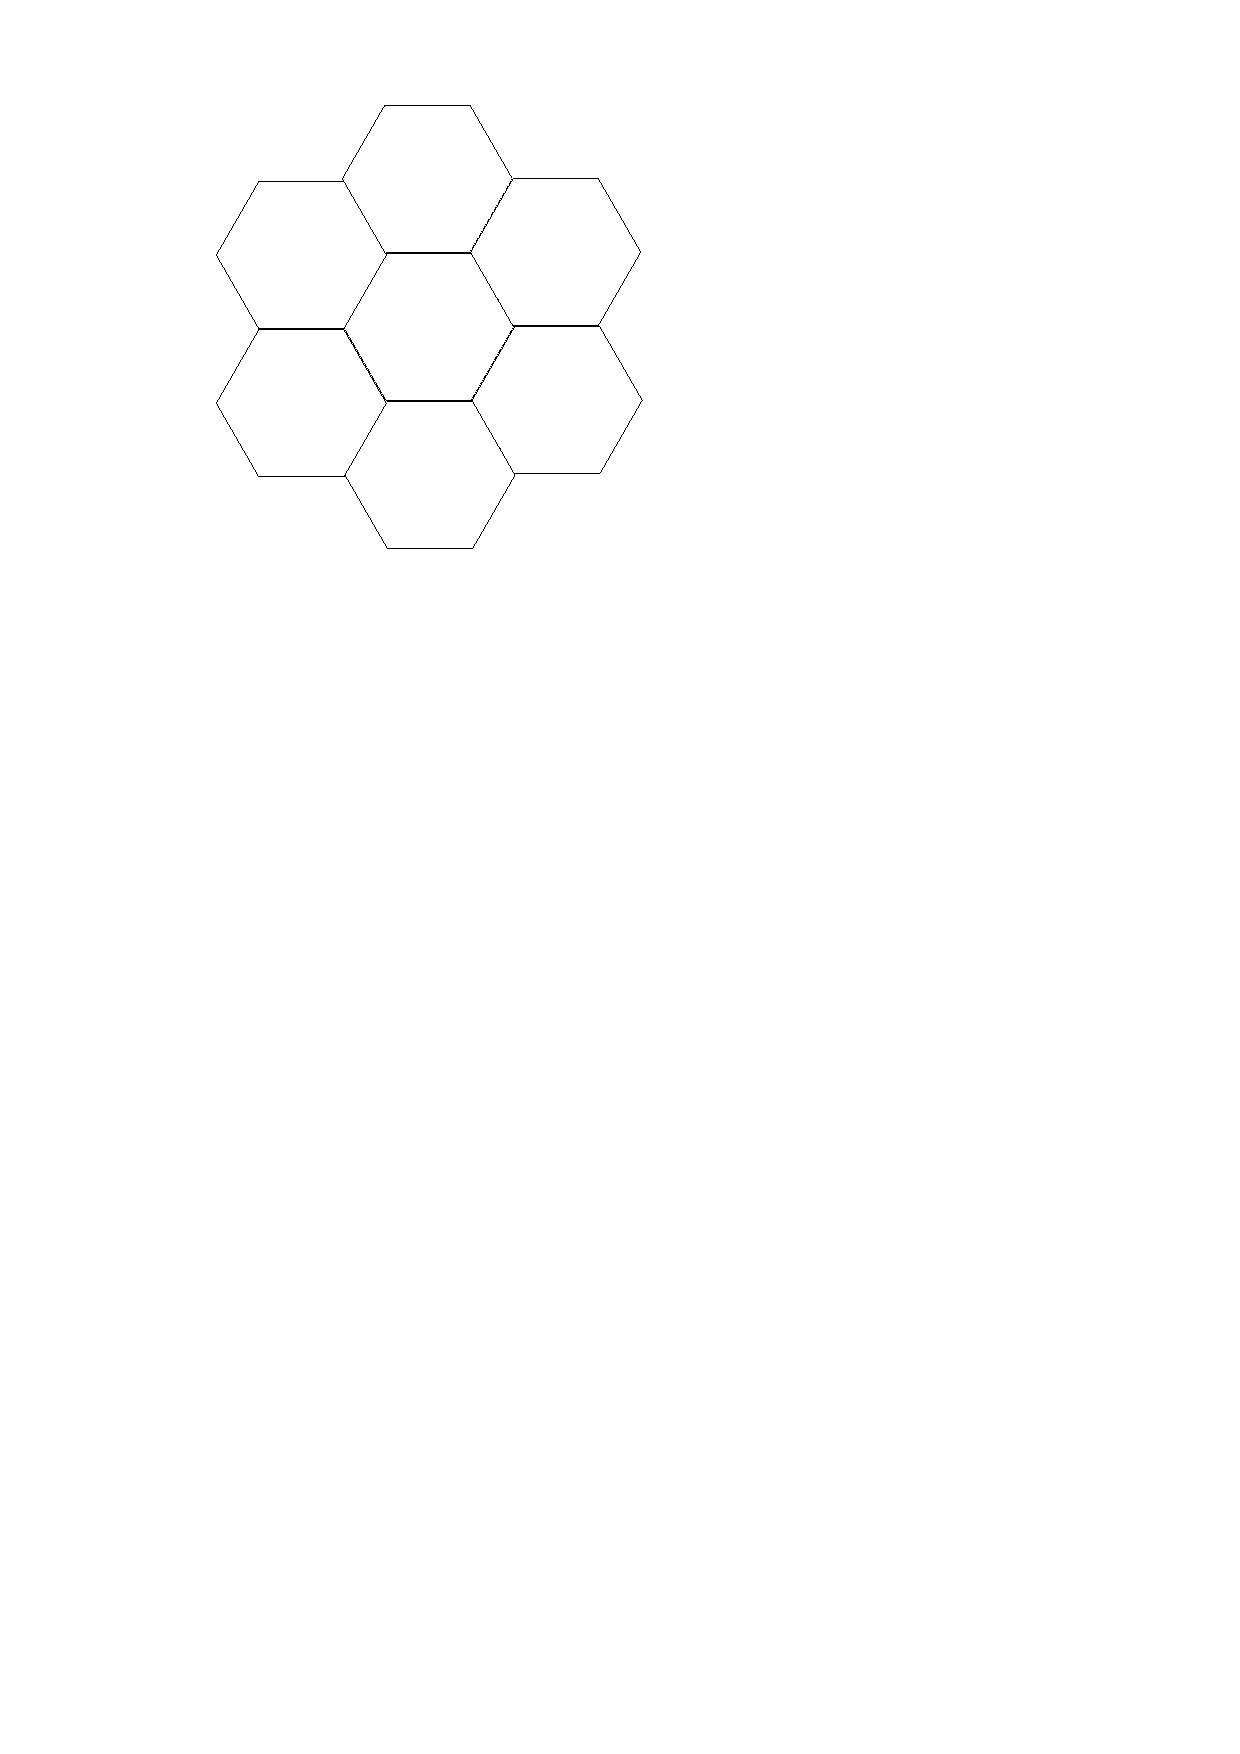
\includegraphics[scale=.33]{graphics/7hexLocked.pdf}
\caption{A locked 7 hexagonal configuration.  (needs to modify picture by
placing red points for hing points.)}
\label{figure:7hexLocked}
\end{center} 
\end{figure}
To prove that it is a locked configuration:
\begin{itemize}
 \item[\rn{1}]
 \item[\rn{2}]
 \item[\rn{3}]
 \item[\rn{4}]
 \item[\rn{5}]
 \item[\rn{6}]
 \item[\rn{7}]
 \item[\rn{8}]
 \item[\rn{9}]
 \item[\rn{10}]
 \end{itemize}
\subsubsection{Hinged Hexagons}
\begin{thm}[]\label{thm}
Any finite collection of polygons of equal area has a common hinged dissection.
\cite{abbott2012hinged}
\end{thm}
\paragraph{The Shapes}
Figure \ref{fig:lockingShape} is a locking shape:
\begin{figure}[h]
\begin{center}
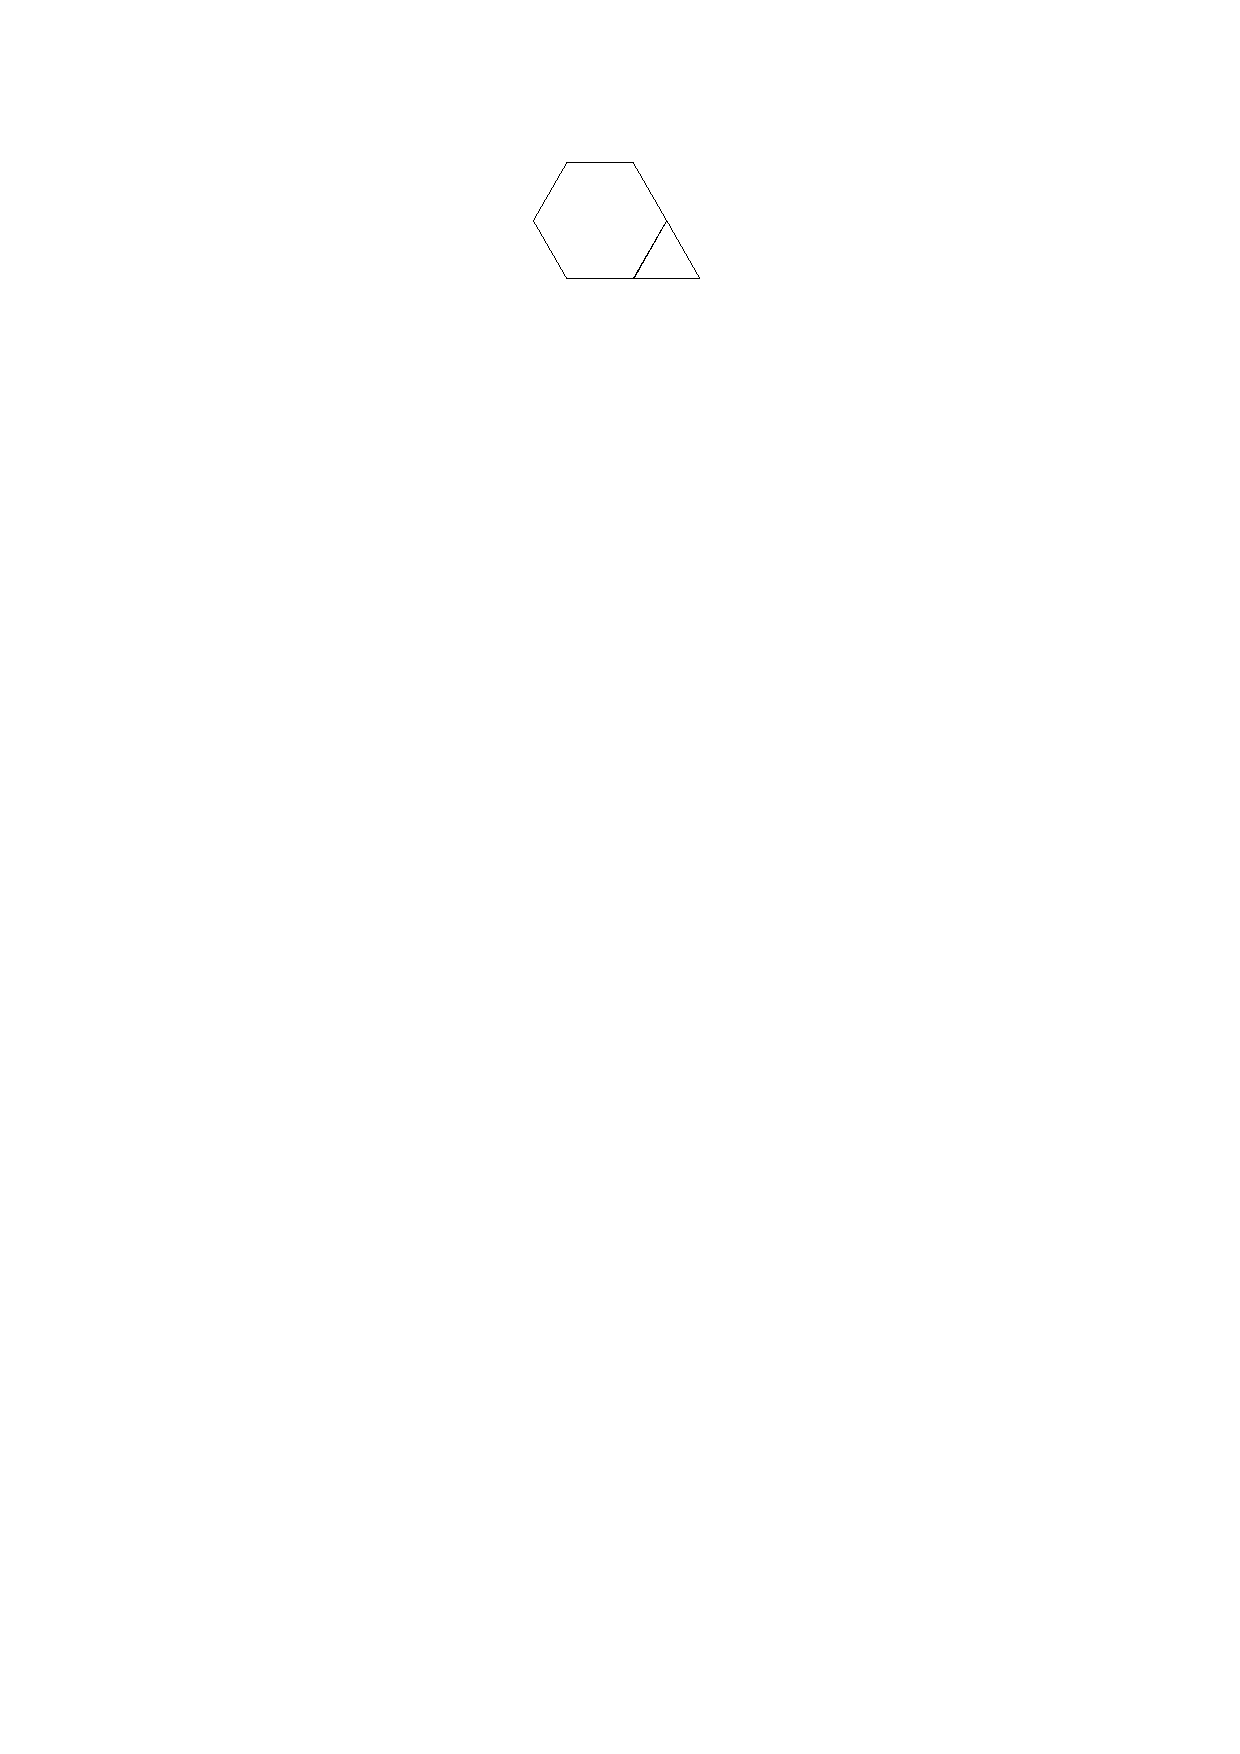
\includegraphics{graphics/lockingShape.pdf}
\caption{This is the shapte that resides in boundary of the lattice.}
\label{fig:lockingShape}
\end{center}
\end{figure}
Figure \ref{fig:lockingShape} shall reside in the boundary of a lattice and have
a hinge point at one vertex where the locking shape and boundary meet.
\begin{figure}[h]
\begin{center}
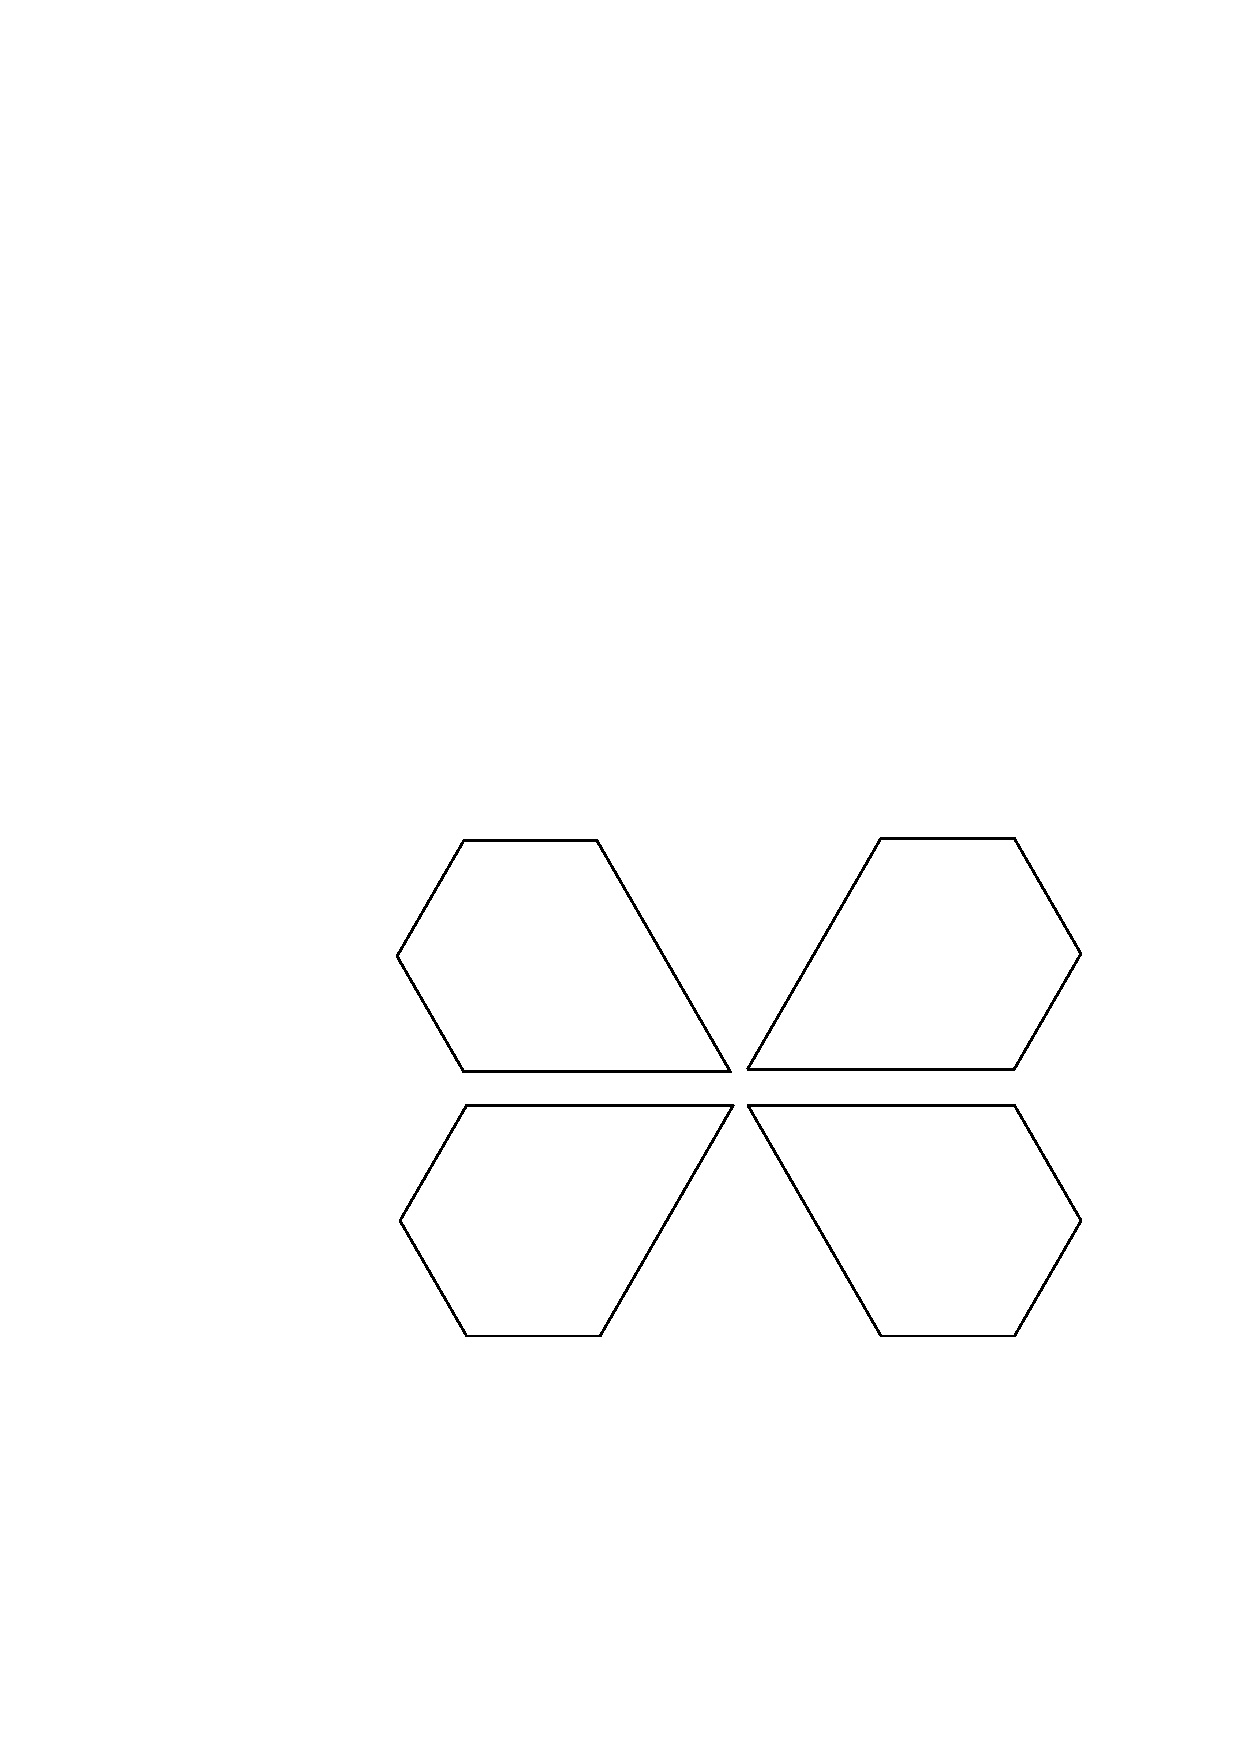
\includegraphics{graphics/shapeInChannel.pdf}
\end{center} 
\caption{A locking shape in the lattice boundary's channel.}
\label{fig:lockingShapeInChannel}
\end{figure}
\paragraph{Junctions}
We define junctions to be the point three hexagons meet in a hexagonal lattice,
e.g. Figure \ref{fig:lattice}.
%Radius of regular polygons 
\newdimen\R
\R=4.5cm
\begin{figure}[h] 
\begin{center}
\begin{tikzpicture}
\begin{scope}
\filldraw[pattern=hexagons]  (0:\R) \foreach \x in {60,120,...,359} {
                -- (\x:\R)
            }-- cycle (90:\R);
\end{scope}
\end{tikzpicture}
\caption{A portion of a hexagonal lattice.}
\label{fig:lattice}
\end{center}
\end{figure}
\newpage
\paragraph{Central Scaling}
\paragraph{Junctions in Conjunctive Normal Form}
Explain the configurations we're interested in.
\subsubsection{Configurations and Locked Configurations}